\documentclass[a4paper,14pt]{extarticle}

\usepackage[utf8x]{inputenc}
\usepackage[T1,T2A]{fontenc}
\usepackage[russian]{babel}
\usepackage{hyperref}
\usepackage{indentfirst}
\usepackage{here}
\usepackage{array}
\usepackage{graphicx}
\usepackage{caption}
\usepackage{subcaption}
\usepackage{chngcntr}
\usepackage{amsmath}
\usepackage{amssymb}
\usepackage{pgfplots}
\usepackage{pgfplotstable}
\usepackage[left=2cm,right=2cm,top=2cm,bottom=2cm,bindingoffset=0cm]{geometry}
\usepackage{multicol}

\renewcommand{\le}{\ensuremath{\leqslant}}
\renewcommand{\leq}{\ensuremath{\leqslant}}
\renewcommand{\ge}{\ensuremath{\geqslant}}
\renewcommand{\geq}{\ensuremath{\geqslant}}
\renewcommand{\epsilon}{\ensuremath{\varepsilon}}
\renewcommand{\phi}{\ensuremath{\varphi}}

\counterwithin{figure}{section}
\counterwithin{equation}{section}
\counterwithin{table}{section}
\newcommand{\sign}[1][5cm]{\makebox[#1]{\hrulefill}} % Поля подписи и даты
\graphicspath{{pics/}} % Путь до папки с картинками
\captionsetup{justification=centering,margin=1cm}
\def\arraystretch{1.3}

\begin{document}	% начало документа

\begin{titlepage}
\begin{center}
	\textbf{Санкт-Петербургский Политехнический Университет \\Петра Великого}\\[0.3cm]
	\small Институт компьютерных наук и технологий \\[0.3cm]
	\small Кафедра компьютерных систем и программных технологий\\[4cm]
	
	\textbf{ОТЧЕТ}\\ \textbf{о лабораторной работе}\\[0.5cm]
	\textbf{<<Исследование частотных характеристик пассивных RC-цепей>>}\\[0.1cm]
	\textbf{Электротехника и Электроника}\\[10.5cm]
\end{center}

\begin{flushright}
	\begin{minipage}{0.60\textwidth}
		\begin{flushleft}
			\small \textbf{Работу выполнили студенты}\\[3mm]
			\small группа 23501/4 \hspace*{17mm} Дьячков В.В.\\[3mm]
			\small группа 23501/4 \hspace*{17mm} Ламтев А.Ю.\\[5mm]
			
			\small \textbf{Преподаватель}\\[5mm]
		 	\small \sign[3.5cm] \hspace*{8mm} к.т.н., доц. Кочетков Ю.Д.\\[0.5cm]
		\end{flushleft}
	\end{minipage}
\end{flushright}

\vfill

\begin{center}
	\small Санкт-Петербург\\
	\small \the\year
\end{center}
\end{titlepage}


\section{Цель работы}

Ознакомиться с принципом действия параметрического стабилизатора напряжения. Настроить и исследовать его. Рассчитать силовые звенья.

\section{Чертеж схемы исследуемого устройства}

\begin{figure}[h]
\centering
\begin{subfigure}[b]{0.45\textwidth}
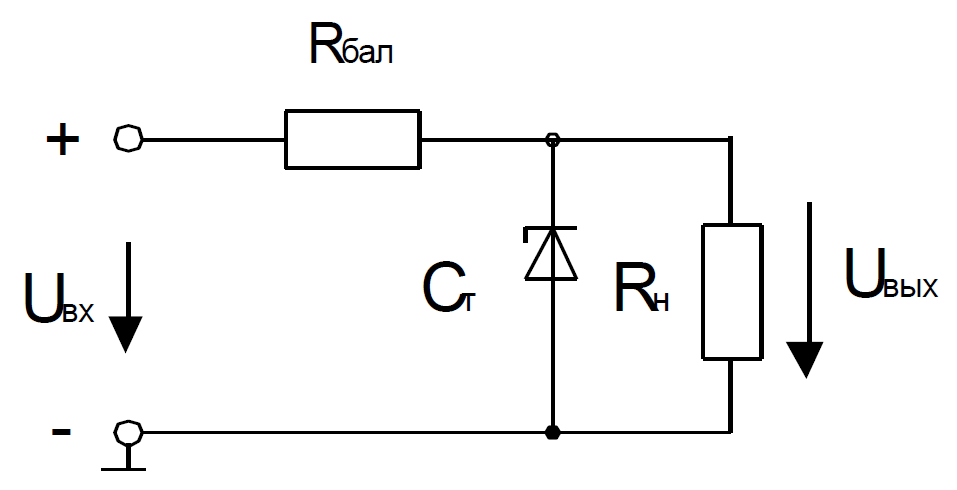
\includegraphics[scale=0.35]{img/stabilizator.png}
\caption{Параметрический стабилизатор\\ постоянного напряжения}\label{figure:2.1:a}
\end{subfigure}
\begin{subfigure}[b]{0.45\textwidth}
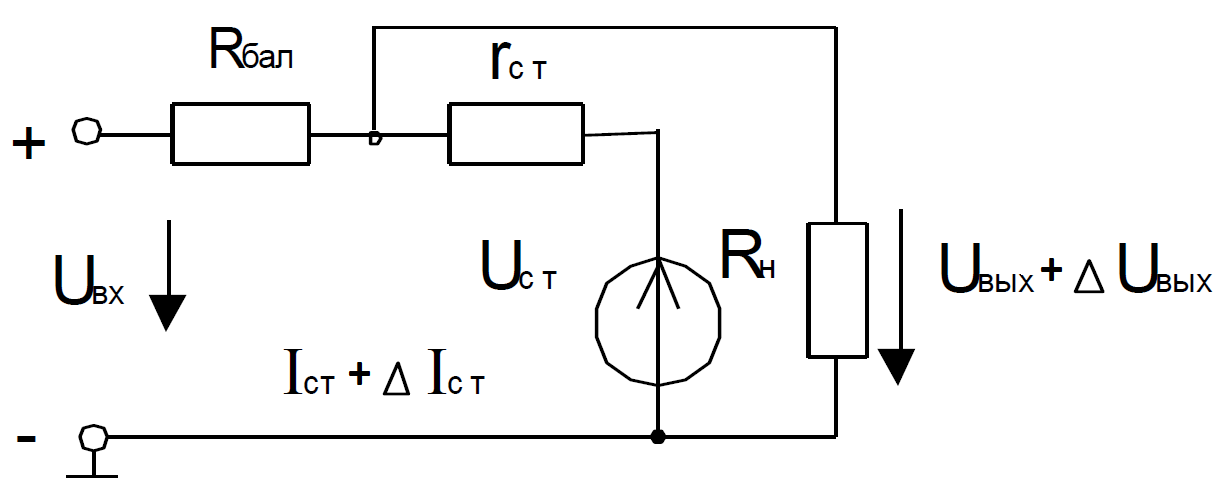
\includegraphics[scale=0.35]{img/substitution.png}
\caption{Схема замещения \\стабилизатора}\label{figure:2.1:b}
\end{subfigure}
\caption{}\label{figure:2.1}
\end{figure}


\section{Исходные данные}

\begin{table}[H]
	\begin{center}
	\caption{Исходные данные}
	\def\arraystretch{1.2}
		\begin{tabular}{|c|c|}
		\hline 
		$U_\text{вх}$ & 15 В \\ 
		\hline 
		$U_\text{вых}$ & 9 В \\ 
		\hline 
		$I_p$ & 8 мА \\ 
		\hline 
		$R_\text{н}$ & 500 Ом \\ 
		\hline 
		\end{tabular} 
		\label{tab:3:1}
	\end{center}
\end{table}

\begin{table}[H]
	\begin{center}
	\caption{Характеристика стабилитрона кс156А}
	\def\arraystretch{1.2}
		\begin{tabular}{|c|c|}
		\hline 
		$U$ & 5.6 В \\ 
		\hline 
		$I_{\text{ст}\ min}$ & 3 мА \\ 
		\hline 
		$I_{\text{ст}\ max}$ & 50 мА \\ 
		\hline 
		$r_{\text{ст}}$ & 46 Ом \\ 
		\hline 
		\end{tabular} 
		\label{tab:3:2}
	\end{center}
\end{table}


\section{Теоретические расчеты и зависимости}

\subsection{Расчет параметров элементов и характеристик стабилизатора}
%\begin{flalign*}
$I_\text{вых} = \frac{U_\text{вых}}{R_\text{н}} = \frac{9}{500} = 0.018$ A
%\end{flalign*}
$R_\text{бал} = \frac{U_\text{вх} - U_\text{вых}}{I_p + I_\text{вых}} = \frac{15 - 9}{0.008 + 0.018} = 230.769$ Ом

$U_{\text{вх}\ min} = U_\text{вых} + R_\text{бал} \cdot (I_{\text{ст}\ min} + I_\text{вых}) = 9 + 230.769 \cdot (0.003 + 0.018) = \\[1mm] = 13.846$ В

$U_{\text{вх}\ max} = U_\text{вых} + R_\text{бал} \cdot (I_{\text{ст}\ max} + I_\text{вых}) = 9 + 230.769 \cdot (0.05 + 0.018) = \\[1mm] = 24.692$ В

$I_{\text{вых}\ min} = 0$

$I_{\text{вых}\ max} = \frac{U_\text{вх} - U_\text{вых} - I_{\text{ст}\ min} \cdot R_\text{бал}}{R_\text{бал}} = \frac{15 - 9 - 0.003 \cdot 230.769}{230.769} = 0.023$ А

$R_{\text{н}\ min} = \frac{U_\text{вых}}{I_{\text{вых}\ max}} = \frac{9}{0.023} = 391$ Ом

$R_{\text{н}\ max} = \frac{U_\text{вых}}{I_{\text{вых}\ min}} = \frac{9}{0} = \infty $ Ом 

\subsection{Расчет коэффициента стабилизации и выходного сопротивления}

\begin{equation}
K_\text{ст} = \frac{R_\text{бал} \cdot U_\text{вых}}{r_\text{ст} \cdot U_\text{вх}}
\end{equation}

\begin{equation}
R_\text{вых} \simeq r_{\text{ст}}
\end{equation}

\begin{flalign*}
K_\text{ст} = \frac{R_\text{бал} \cdot U_\text{вых}}{r_\text{ст} \cdot U_\text{вх}} = \frac{230.769 \cdot 9}{46 \cdot 15} = 3.01
\end{flalign*}

\begin{flalign*}
R_\text{вых} \simeq r_{\text{ст}} < 46\ \ \text{Ом}
\end{flalign*}

\section{Экспериментально снятые зависимости}

\begin{table}[H]
	\begin{center}
	\caption{Зависимость $U_\text{вых} = f(U_\text{вх})$}
	\def\arraystretch{1.2}
		\begin{tabular}{|c|c|}
		\hline 
		$U_\text{вх}$, В & $U_\text{вых}$, В \\ 
		\hline 
		1.091 & 0.696 \\ 
		\hline 
		2.98 & 1.90 \\ 
		\hline 
		4.97 & 3.17 \\ 
		\hline 
		6.99 & 4.35 \\ 
		\hline %началась стабилизация, ура!!! 
		9.04 & 5.00 \\ 
		\hline 
		11.05 & 5.23 \\ 
		\hline 
		13.03 & 5.33 \\ 
		\hline 
		15.00 & 5.40 \\ 
		\hline 
		16.96 & 5.45 \\ 
		\hline 
		19.02 & 5.50 \\ 
		\hline 
		21.00 & 5.53 \\ 
		\hline 
		23.00 & 5.56 \\ 
		\hline 
		24.6 & 5.58 \\ 
		\hline 
		\end{tabular} 
		\label{tab:5:1}
	\end{center}
\end{table}

\begin{figure}[H]
	\begin{center}
		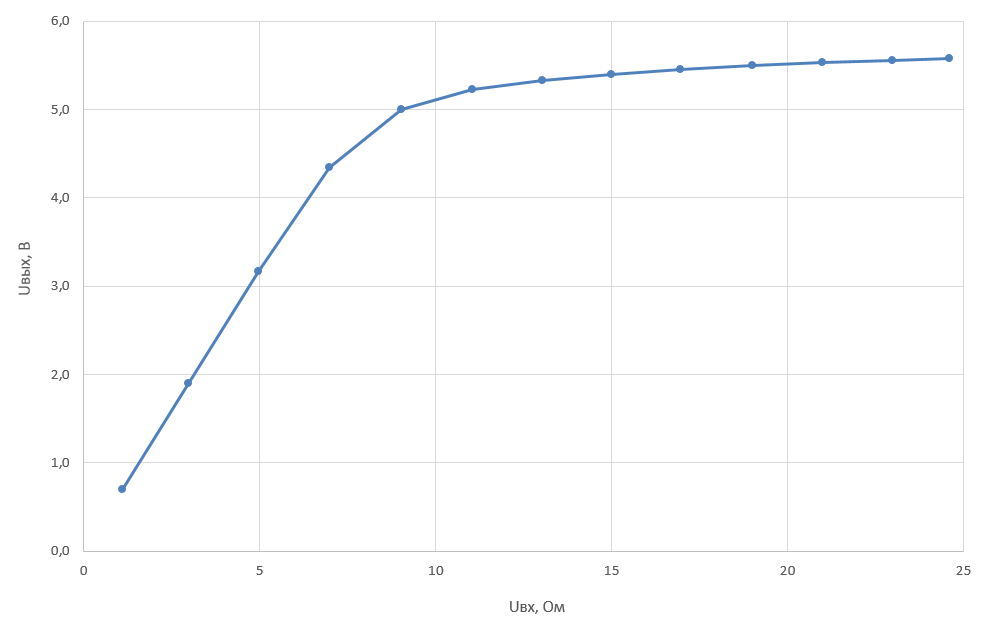
\includegraphics[width=14cm]{img/Uout(Uin).png}
		\caption{Зависимость $U_\text{вых} = f(U_\text{вх})$}
		\label{graphic:5:1} % название для ссылок внутри кода
	\end{center}
\end{figure}

\begin{flalign*}
K_\text{ст} = \frac{\Delta U_\text{вх}}{\Delta U_\text{ст}} = \frac{24.60 - 11.05}{5.58 - 5.23} = 38,72
\end{flalign*}

\begin{table}[H]
	\begin{center}
	\caption{Зависимость $U_\text{вых} = f(R_\text{н})$}
	\def\arraystretch{1.2}
		\begin{tabular}{|c|c|c|}
		\hline 
		$R_\text{н}$, Ом & $U_\text{вых}$, В & $I_\text{н}$, мА\\ 
		\hline
		10 & 0.54 & 59.60 \\ 
		\hline 
		20 & 1.12 & 55.85 \\ 
		\hline 
		43 & 2.11 & 49.07 \\ 
		\hline 
		63.00 & 2.81 & 44.60 \\ 
		\hline 
		82.00 & 3.37 & 41.10 \\ 
		\hline 
		121.00 & 4.33 & 35.79 \\ 
		\hline 
		159.11 & 4.82 & 30.29 \\ 
		\hline 
		222.18 & 5.25 & 23.63 \\ 
		\hline 
		248.12 & 5.30 & 21.36 \\ 
		\hline 
		283.26 & 5.32 & 18.78 \\ 
		\hline 
		330.00 & 5.35 & 16.21 \\  
		\hline 
		404.76 & 5.38 & 13.29 \\ 
		\hline 
		507.46 & 5.40 & 10.64 \\ 
		\hline 
		609.04 & 5.41 & 8.88 \\ 
		\hline 
		795.92 & 5.44 & 6.83 \\ 
		\hline   
		970.59 & 5.45 & 5.62 \\ 
		\hline 
		1322.03 & 5.46 & 4.13 \\ 
		\hline 
		1885.71 & 5.46 & 2.90 \\ 
		\hline
		1942.86 & 5.47 & 2.82 \\ 
		\hline 
		\end{tabular} 
		\label{tab:5:2}
	\end{center}
\end{table}

\begin{figure}[H]
	\begin{center}
		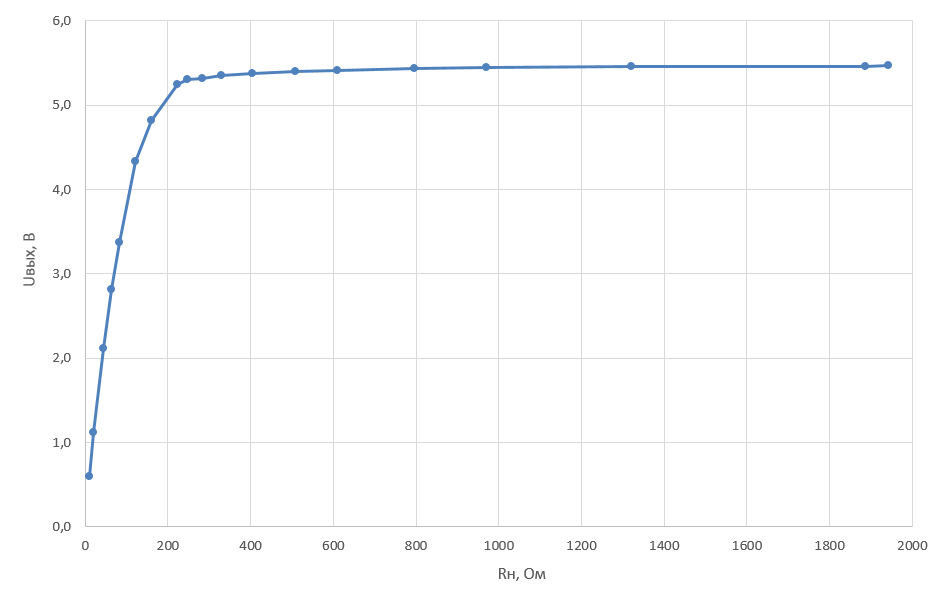
\includegraphics[width=14cm]{img/Uout(Rn).png}
		\caption{График зависимости $U_\text{вых} = f(R_\text{н})$}
		\label{graphic:5:2} % название для ссылок внутри кода
	\end{center}
\end{figure}

\begin{figure}[H]
	\begin{center}
		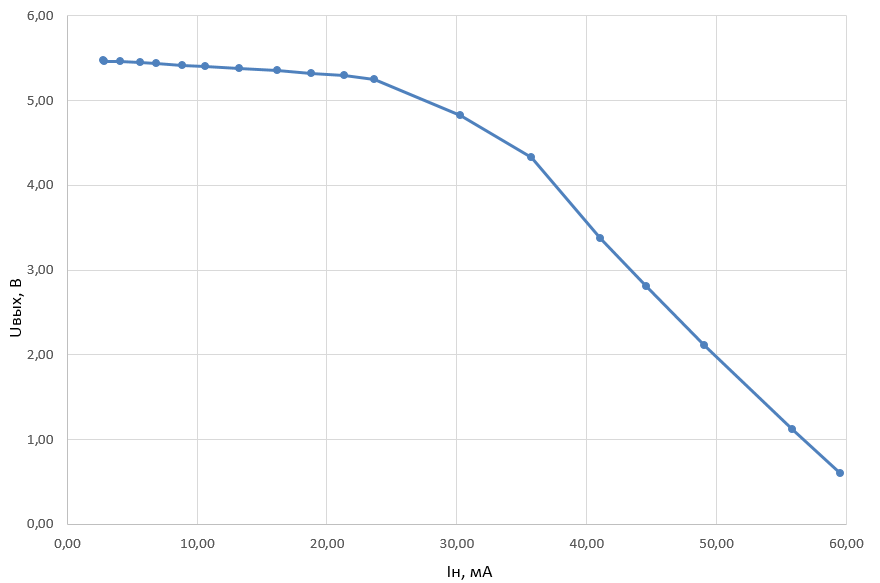
\includegraphics[width=14cm]{img/Uout(In).png}
		\caption{График зависимости $U_\text{вых} = f(I_\text{н})$}
		\label{graphic:5:3} % название для ссылок внутри кода
	\end{center}
\end{figure}

\begin{flalign*}
R_\text{вых} = \frac{\Delta U_\text{ст}}{\Delta I_\text{н}} = \frac{5.47 - 5.25}{(23.63 - 2.82) \cdot 10^{-3}} = 10.57 \ \ \text{Ом}
\end{flalign*}

\section{Анализ экспериментальных вычислений}

$R_\text{вых\ \ эксп} = 10.57 $ Ом $< R_\text{вых\ \ теор} < r_\text{ст} < 46$ Ом

$K_\text{ст} \sim \frac{1}{r_\text{ст}} \Rightarrow K_\text{ст\ \ эксп}$ должно быть $> K_\text{ст\ \ теор} = 3.01$

$K_\text{ст\ \ эксп} = 38.72 > K_\text{ст\ \ теор} = 3.01$

\section{Выводы}

Вычисленное значение $R_\text{вых}$ не превосходит предельно допустимое, и вычисленное значение $K_\text{ст}$ больше, чем минимально допустимое.

Таким образом, формулы для вычисления теоретических значений $K_\text{ст}$ и $R_\text{вых}$ 4.1 и 4.2 являются верными.

\end{document}
